% Options for packages loaded elsewhere
\PassOptionsToPackage{unicode}{hyperref}
\PassOptionsToPackage{hyphens}{url}
%
\documentclass[
  ignorenonframetext,
]{beamer}
\usepackage{pgfpages}
\setbeamertemplate{caption}[numbered]
\setbeamertemplate{caption label separator}{: }
\setbeamercolor{caption name}{fg=normal text.fg}
\beamertemplatenavigationsymbolsempty
% Prevent slide breaks in the middle of a paragraph
\widowpenalties 1 10000
\raggedbottom
\setbeamertemplate{part page}{
  \centering
  \begin{beamercolorbox}[sep=16pt,center]{part title}
    \usebeamerfont{part title}\insertpart\par
  \end{beamercolorbox}
}
\setbeamertemplate{section page}{
  \centering
  \begin{beamercolorbox}[sep=12pt,center]{part title}
    \usebeamerfont{section title}\insertsection\par
  \end{beamercolorbox}
}
\setbeamertemplate{subsection page}{
  \centering
  \begin{beamercolorbox}[sep=8pt,center]{part title}
    \usebeamerfont{subsection title}\insertsubsection\par
  \end{beamercolorbox}
}
\AtBeginPart{
  \frame{\partpage}
}
\AtBeginSection{
  \ifbibliography
  \else
    \frame{\sectionpage}
  \fi
}
\AtBeginSubsection{
  \frame{\subsectionpage}
}
\usepackage{lmodern}
\usepackage{amssymb,amsmath}
\usepackage{ifxetex,ifluatex}
\ifnum 0\ifxetex 1\fi\ifluatex 1\fi=0 % if pdftex
  \usepackage[T1]{fontenc}
  \usepackage[utf8]{inputenc}
  \usepackage{textcomp} % provide euro and other symbols
\else % if luatex or xetex
  \usepackage{unicode-math}
  \defaultfontfeatures{Scale=MatchLowercase}
  \defaultfontfeatures[\rmfamily]{Ligatures=TeX,Scale=1}
\fi
% Use upquote if available, for straight quotes in verbatim environments
\IfFileExists{upquote.sty}{\usepackage{upquote}}{}
\IfFileExists{microtype.sty}{% use microtype if available
  \usepackage[]{microtype}
  \UseMicrotypeSet[protrusion]{basicmath} % disable protrusion for tt fonts
}{}
\makeatletter
\@ifundefined{KOMAClassName}{% if non-KOMA class
  \IfFileExists{parskip.sty}{%
    \usepackage{parskip}
  }{% else
    \setlength{\parindent}{0pt}
    \setlength{\parskip}{6pt plus 2pt minus 1pt}}
}{% if KOMA class
  \KOMAoptions{parskip=half}}
\makeatother
\usepackage{xcolor}
\IfFileExists{xurl.sty}{\usepackage{xurl}}{} % add URL line breaks if available
\IfFileExists{bookmark.sty}{\usepackage{bookmark}}{\usepackage{hyperref}}
\hypersetup{
  pdftitle={305 Lecture 14 - Explosion},
  pdfauthor={Brian Weatherson},
  hidelinks,
  pdfcreator={LaTeX via pandoc}}
\urlstyle{same} % disable monospaced font for URLs
\newif\ifbibliography
\usepackage{graphicx,grffile}
\makeatletter
\def\maxwidth{\ifdim\Gin@nat@width>\linewidth\linewidth\else\Gin@nat@width\fi}
\def\maxheight{\ifdim\Gin@nat@height>\textheight\textheight\else\Gin@nat@height\fi}
\makeatother
% Scale images if necessary, so that they will not overflow the page
% margins by default, and it is still possible to overwrite the defaults
% using explicit options in \includegraphics[width, height, ...]{}
\setkeys{Gin}{width=\maxwidth,height=\maxheight,keepaspectratio}
% Set default figure placement to htbp
\makeatletter
\def\fps@figure{htbp}
\makeatother
\setlength{\emergencystretch}{3em} % prevent overfull lines
\providecommand{\tightlist}{%
  \setlength{\itemsep}{0pt}\setlength{\parskip}{0pt}}
\setcounter{secnumdepth}{-\maxdimen} % remove section numbering
\let\Tiny=\tiny

 \setbeamertemplate{navigation symbols}{} 

% \usetheme{Madrid}
 \usetheme[numbering=none, progressbar=foot]{metropolis}
 \usecolortheme{wolverine}
 \usepackage{color}
 \usepackage{MnSymbol}
% \usepackage{movie15}

\usepackage{amssymb}% http://ctan.org/pkg/amssymb
\usepackage{pifont}% http://ctan.org/pkg/pifont
\newcommand{\cmark}{\ding{51}}%
\newcommand{\xmark}{\ding{55}}%

\DeclareSymbolFont{symbolsC}{U}{txsyc}{m}{n}
\DeclareMathSymbol{\boxright}{\mathrel}{symbolsC}{128}
\DeclareMathAlphabet{\mathpzc}{OT1}{pzc}{m}{it}


% \usepackage{tikz-qtree}
% \usepackage{markdown}
% \usepackage{prooftrees}
% \forestset{not line numbering, close with = x}
% Allow for easy commas inside trees
\renewcommand{\,}{\text{, }}


\usepackage{tabulary}

\usepackage{open-logic-config}

\setlength{\parskip}{1ex plus 0.5ex minus 0.2ex}

\AtBeginSection[]
{
\begin{frame}
	\Huge{\color{darkblue} \insertsection}
\end{frame}
}

\renewenvironment*{quote}	
	{\list{}{\rightmargin   \leftmargin} \item } 	
	{\endlist }

\definecolor{darkgreen}{rgb}{0,0.7,0}
\definecolor{darkblue}{rgb}{0,0,0.8}

\newcommand{\starttab}{\begin{center}
\vspace{6pt}
\begin{tabular}}

\newcommand{\stoptab}{\end{tabular}
\vspace{6pt}
\end{center}
\noindent}


\newcommand{\sif}{\rightarrow}
\newcommand{\siff}{\leftrightarrow}
\newcommand{\EF}{\end{frame}}


\newcommand{\TreeStart}[1]{
%\end{frame}
\begin{frame}
\begin{center}
\begin{tikzpicture}[scale=#1]
\tikzset{every tree node/.style={align=center,anchor=north}}
%\Tree
}

\newcommand{\TreeEnd}{
\end{tikzpicture}
%\end{center}
}

\newcommand{\DisplayArg}[2]{
\begin{enumerate}
{#1}
\end{enumerate}
\vspace{-6pt}
\hrulefill

%\hspace{14pt} #2
%{\addtolength{\leftskip}{14pt} #2}
\begin{quote}
{\normalfont #2}
\end{quote}
\vspace{12pt}
}

\newenvironment{ProofTree}[1][1]{
\begin{center}
\begin{tikzpicture}[scale=#1]
\tikzset{every tree node/.style={align=center,anchor=south}}
}
{
\end{tikzpicture}
\end{center}
}

\newcommand{\TreeFrame}[2]{
\begin{columns}[c]
\column{0.5\textwidth}
\begin{center}
\begin{prooftree}{}
#1
\end{prooftree}
\end{center}
\column{0.45\textwidth}
%\begin{markdown}
#2
%\end{markdown}
\end{columns}
}

\newcommand{\ScaledTreeFrame}[3]{
\begin{columns}[c]
\column{0.5\textwidth}
\begin{center}
\scalebox{#1}{
\begin{prooftree}{}
#2
\end{prooftree}
}
\end{center}
\column{0.45\textwidth}
%\begin{markdown}
#3
%\end{markdown}
\end{columns}
}

\usepackage[bb=boondox]{mathalfa}
\DeclareMathAlphabet{\mathbx}{U}{BOONDOX-ds}{m}{n}
\SetMathAlphabet{\mathbx}{bold}{U}{BOONDOX-ds}{b}{n}
\DeclareMathAlphabet{\mathbbx} {U}{BOONDOX-ds}{b}{n}

\RequirePackage{bussproofs}
\RequirePackage[tableaux]{prooftrees}

\newenvironment{oltableau}{\center\tableau{}} %wff format={anchor = base west}}}
       {\endtableau\endcenter}
       
\newcommand{\formula}[1]{$#1$}

\usepackage{tabulary}
\usepackage{booktabs}

\def\begincols{\begin{columns}}
\def\begincol{\begin{column}}
\def\endcol{\end{column}}
\def\endcols{\end{columns}}

\usepackage[italic]{mathastext}
\usepackage{nicefrac}

\definecolor{mygreen}{RGB}{0, 100, 0}
\definecolor{mypink2}{RGB}{219, 48, 122}
\definecolor{dodgerblue}{RGB}{30,144,255}

\def\True{\textcolor{dodgerblue}{\text{T}}}
\def\False{\textcolor{red}{\text{F}}}

\title{305 Lecture 14 - Explosion}
\author{Brian Weatherson}
\date{July 8, 2020}

\begin{document}
\frame{\titlepage}

\begin{frame}{Plan for Today}
\protect\hypertarget{plan-for-today}{}

\begin{itemize}
\tightlist
\item
  We're going to talk two interesting consequences of the rules we've
  produced so far.
\item
  The first is that the rules validate explosion, the idea that
  everything follows from a contradiction.
\item
  The second is that they validate all four of what are called
  DeMorgan's Laws.
\end{itemize}

\end{frame}

\begin{frame}{Associated Reading}
\protect\hypertarget{associated-reading}{}

No associated reading, but again, this will be relevant to our later
work.

\end{frame}

\hypertarget{explosion}{%
\section{Explosion}\label{explosion}}

\begin{frame}{What It is}
\protect\hypertarget{what-it-is}{}

\(P, \neg P \vdash Q\)

\end{frame}

\begin{frame}{One Weird Thing About it}
\protect\hypertarget{one-weird-thing-about-it}{}

It violates \textbf{relevance} - the constraint that any valid argument
should have at least some term in common between premise and conclusion.

\end{frame}

\begin{frame}{Informal Argument}
\protect\hypertarget{informal-argument}{}

\begin{itemize}[<+->]
\tightlist
\item
  An argument is valid if it is impossible for the premises to be true
  and the conclusion false.
\item
  In \textbf{Explosion}, it is impossible for the premises to be true.
\item
  So in \textbf{Explosion}, it is impossible for the premises to be true
  and the conclusion false.
\item
  So \textbf{Explosion} is valid.
\end{itemize}

\end{frame}

\begin{frame}{Formal Argument}
\protect\hypertarget{formal-argument}{}

Prove \textbf{Explosion} in Carnap.

\end{frame}

\begin{frame}{First Attempt}
\protect\hypertarget{first-attempt}{}

\begin{figure}
\centering
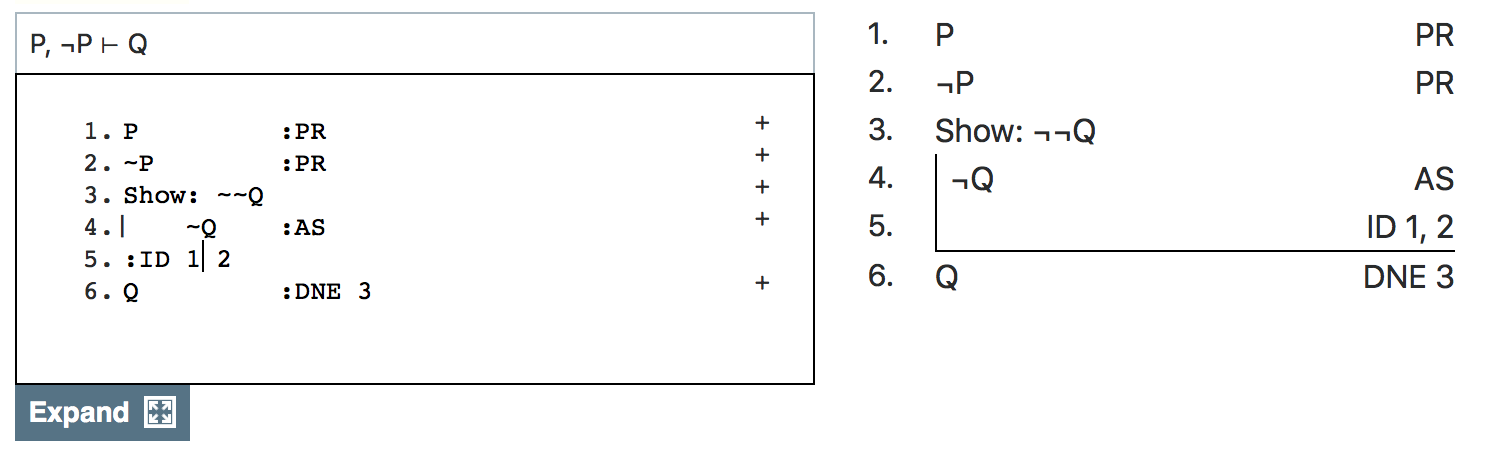
\includegraphics{../images/class05/Class-05-5.png}
\caption{\(P, \neg P \vdash Q\)}
\end{figure}

\end{frame}

\begin{frame}{Second Attempt}
\protect\hypertarget{second-attempt}{}

\begin{figure}
\centering
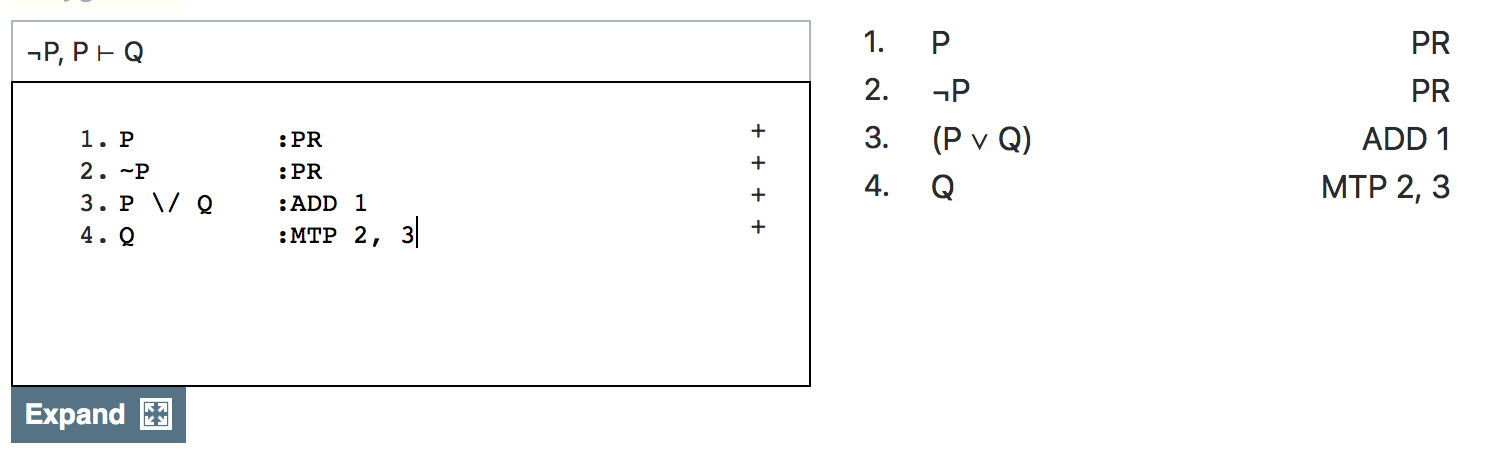
\includegraphics{../images/class05/Class-05-6.png}
\caption{\(P, \neg P \vdash Q\)}
\end{figure}

\end{frame}

\begin{frame}{Choice Point}
\protect\hypertarget{choice-point}{}

\begin{enumerate}
\tightlist
\item
  Reject Addition
\item
  Reject Disjunctive Syllogism
\item
  Accept Explosion
\end{enumerate}

\begin{itemize}[<+->]
\tightlist
\item
  Most people who reject explosion also reject disjunctive syllogism.
\end{itemize}

\end{frame}

\begin{frame}{Why Reject Explosion}
\protect\hypertarget{why-reject-explosion}{}

\begin{enumerate}[<+->]
\tightlist
\item
  Truth in a Database
\item
  Truth in a Story
\item
  There are actual true contradictions, but some things are not true.
\end{enumerate}

\end{frame}

\begin{frame}{My View}
\protect\hypertarget{my-view}{}

Explosion is fine - we just have to be careful with databases and
stories.

\end{frame}

\hypertarget{demorgan-laws}{%
\section{DeMorgan Laws}\label{demorgan-laws}}

\begin{frame}{First Equivalence}
\protect\hypertarget{first-equivalence}{}

\begin{enumerate}
\tightlist
\item
  \(\neg (P \vee Q)\)
\item
  \(\neg P \wedge \neg Q\)
\end{enumerate}

Prove these are equivalent.

\end{frame}

\begin{frame}{First Direction}
\protect\hypertarget{first-direction}{}

\begin{figure}
\centering
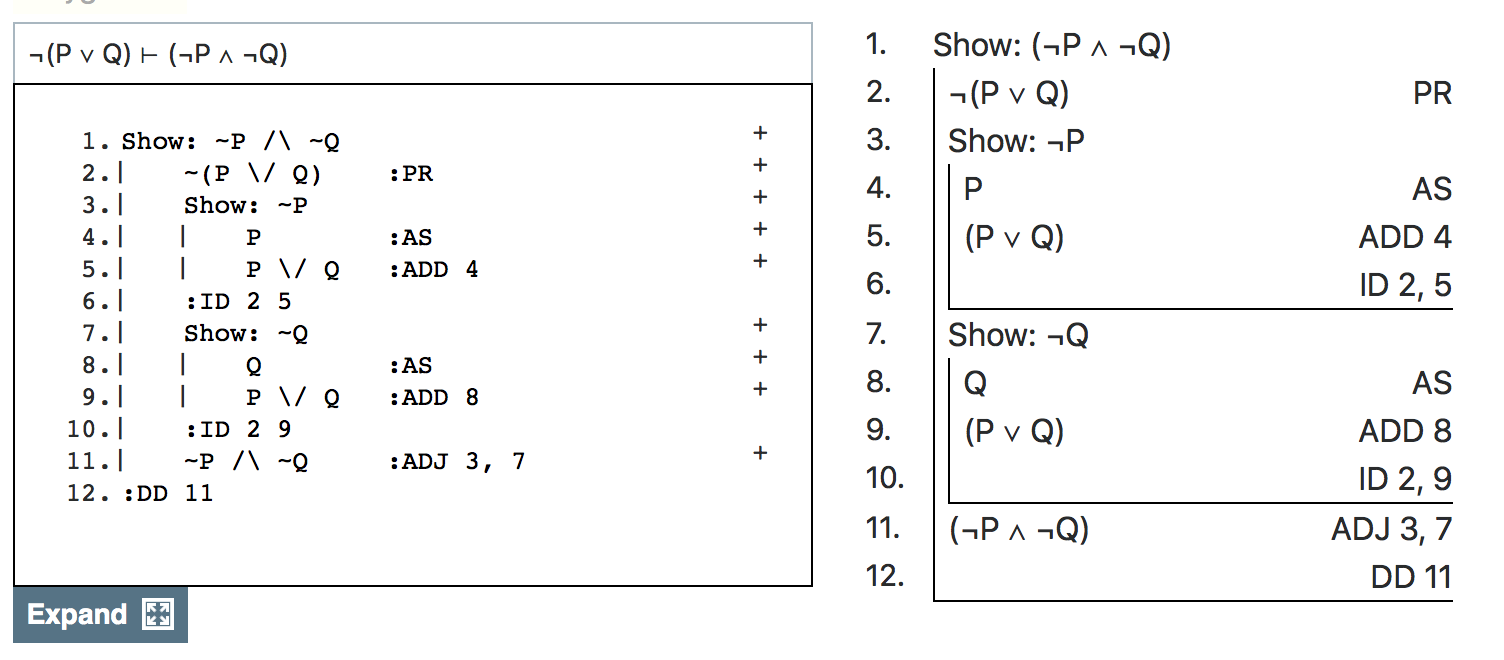
\includegraphics{../images/class05/Class-05-7.png}
\caption{\(\neg (P \vee Q) \vdash \neg P \wedge \neg Q\)}
\end{figure}

\end{frame}

\begin{frame}{Second Direction}
\protect\hypertarget{second-direction}{}

\begin{figure}
\centering
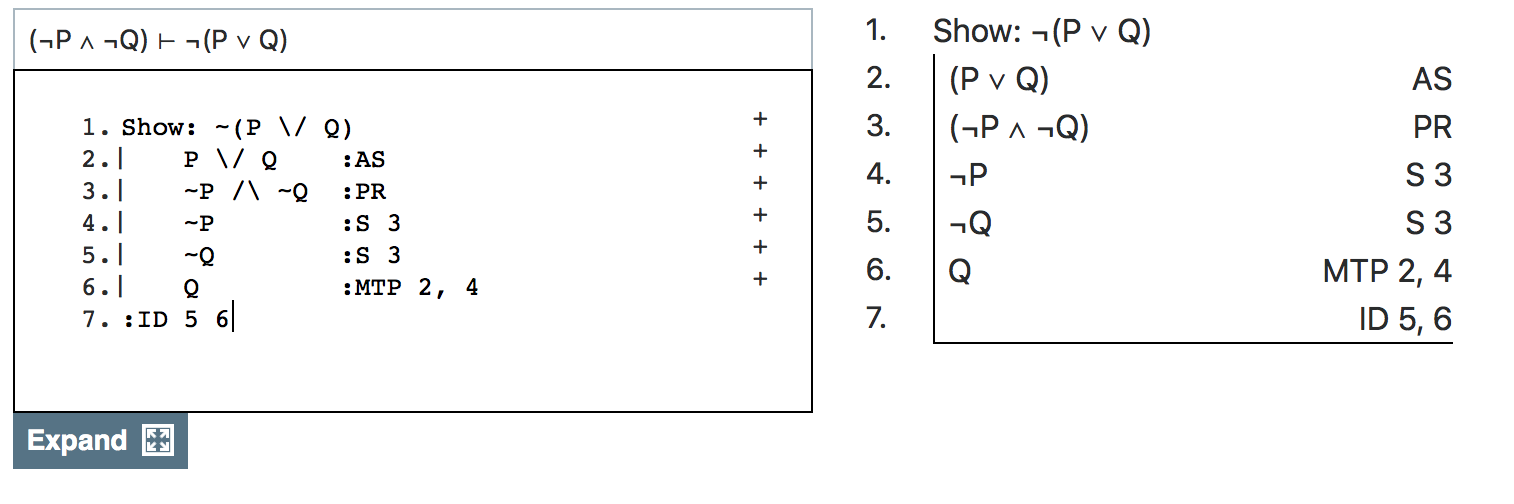
\includegraphics{../images/class05/Class-05-8.png}
\caption{\(\neg P \wedge \neg Q \vdash \neg (P \vee Q)\)}
\end{figure}

\end{frame}

\begin{frame}{Second Equivalence}
\protect\hypertarget{second-equivalence}{}

\begin{enumerate}
\tightlist
\item
  \(\neg P \vee \neg Q\)
\item
  \(\neg (P \wedge Q)\)
\end{enumerate}

\end{frame}

\begin{frame}{First Direction}
\protect\hypertarget{first-direction-1}{}

\begin{figure}
\centering
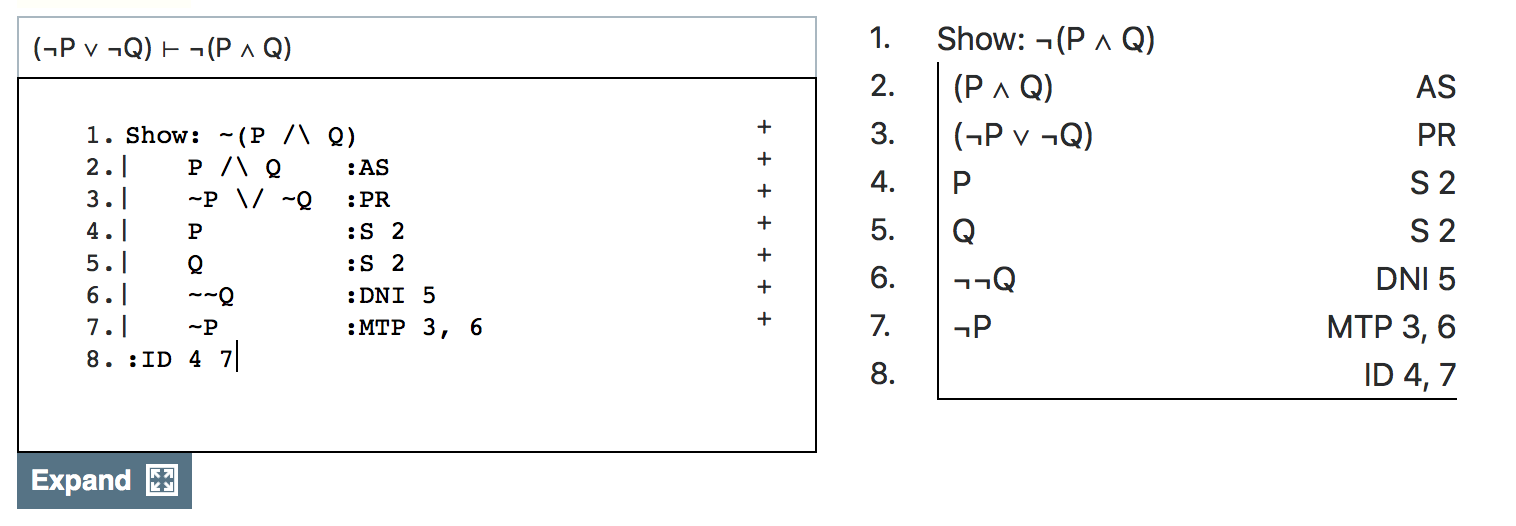
\includegraphics{../images/class05/Class-05-9.png}
\caption{\(\neg (P \wedge Q) \vdash \neg P \vee \neg Q\)}
\end{figure}

\end{frame}

\begin{frame}{Second Direction}
\protect\hypertarget{second-direction-1}{}

\begin{figure}
\centering
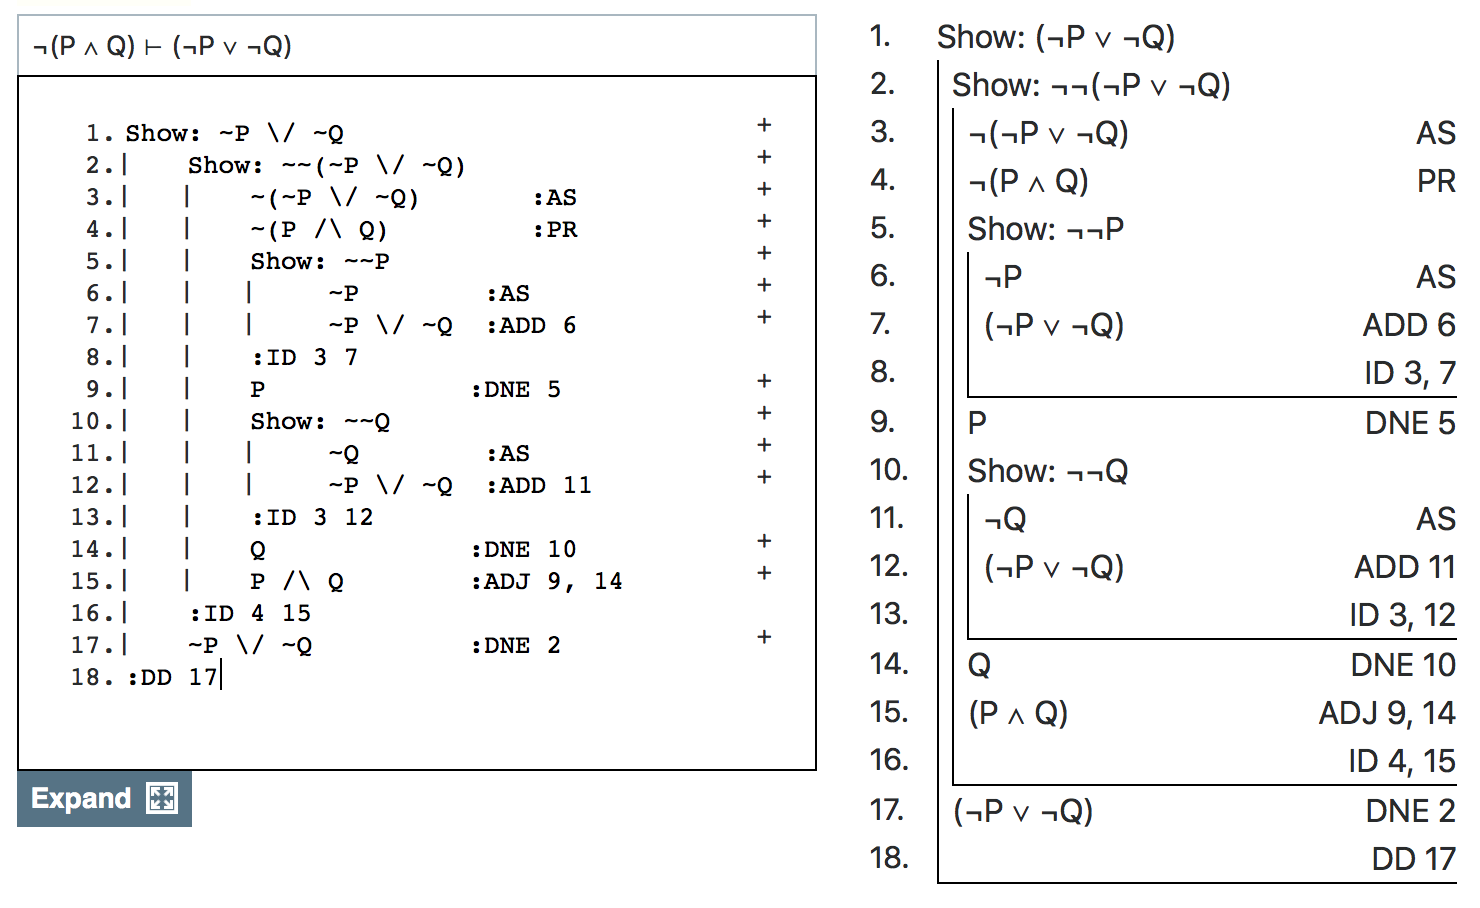
\includegraphics{../images/class05/Class-05-10.png}
\caption{\(\neg (P \wedge Q) \vdash \neg P \vee \neg Q\)}
\end{figure}

\end{frame}

\begin{frame}{General Principle}
\protect\hypertarget{general-principle}{}

To move a negation from outside the parentheses to inside it, you do two
things.

\begin{enumerate}
\tightlist
\item
  Negate each of the parts.
\item
  Flip the conjunction/disjunction symbol upside down.
\end{enumerate}

This process is reversible.

\end{frame}

\begin{frame}{For Next Time}
\protect\hypertarget{for-next-time}{}

Do the weekly assignment, and we'll start talking about truth tables.

\end{frame}

\end{document}
